\section{Grid creation}
\label{section:grid-creation}


\chapterDescription
  {
    15 minutes for the programming but perhaps around 30 minutes for the
    visualisation.
  }
  {
    Chapter \ref{chapter:quickstart}.
  }


In this section, we study a 2d example.
Please adopt your makefile accordingly.
Furthermore, we use the files \texttt{VTKMultilevelGridVisualiserHeader} and
\texttt{...Implementation} as well as
\texttt{VTK2dTreeVisualiser...}.
If you have downloaded the whole Peano repository, these files can be found in
\texttt{pdt/usrtemplates}.
If not, you have to download them manually from the webpage.
Please set up an empty project as discussed in Chapter
\ref{chapter:quickstart} and implement one operation as follows (all other
operations can remain empty/only filled with log statements):


\begin{code}
void myproject::mappings::CreateGrid::touchVertexLastTime(
      myproject::Vertex&               fineGridVertex,
      const tarch::la::Vector<DIMENSIONS,double>&                          fineGridX,
      const tarch::la::Vector<DIMENSIONS,double>&                          fineGridH,
      myproject::Vertex * const        coarseGridVertices,
      const peano::grid::VertexEnumerator&                coarseGridVerticesEnumerator,
      myproject::Cell&                 coarseGridCell,
      const tarch::la::Vector<DIMENSIONS,int>&                             fineGridPositionOfVertex
) {
  logTraceInWith6Arguments( "touchVertexFirstTime(...)", fineGridVertex, fineGridX, ...

  if (
    coarseGridVerticesEnumerator.getLevel()<5
    &&
    tarch::la::equals( fineGridX, 0.0 )
    &&
    fineGridVertex.getRefinementControl()==Vertex::Records::Unrefined
  ) {
    fineGridVertex.refine();
  }

  logTraceOutWith1Argument( "touchVertexFirstTime(...)", fineGridVertex );
}

\end{code}


\noindent
This source fragment requires some additional explanation. 
We neglect the enumerator stuff for the time being.
That will become clear later throughout the present chapter.
The refinement control check says `well, refine, but do it only on unrefined
vertices'.
It's just a matter of good style, not to call \texttt{refine} on a refined
vertex.
The middle line uses a function from the tarch's linear algebra namespace. 
It takes the \texttt{fineGridX} vector (the position of the vertex in space) and
checks whether all entries equal zero.
As we are working with floating point numbers, it is not a bit-wise check. 
Instead, it uses an interval of machine precision around zero.
You may want to change this notion of machine precision in Peano (file
\texttt{Scalar} within the \texttt{tarch::la} namespace). 
In general, it would be a good idea to study the content of the \texttt{la}
component soon---there's lots of useful stuff in there to work with
tiny, dense vectors\footnote{Peano someday should perhaps be rewritten to use
boost linear algebra (\url{http://www.boost.org}) or some fancy template
library.
Feel free to do so.
Right at the moment, it is all plain hand-craftet routines.}.

\begin{remark}
  Peano realises a {\textbf vertex-based}, {\textbf logical-or} refinement: You can
  invoke \texttt{refine} on any unrefined vertex. Peano then refines all cells
  around a vertex in the present or next traversal (it basically tries to do it
  asap, but sometimes data consistency constraints require it to postpone the
  actual refinement by one iteration). The other way round, you may read it as
  follows: A cell is refined if the refinement flag is set for any adjacent
  vertex.
\end{remark}



\begin{remark}
  There is a pitfall induced by the above explanation: Users typically
  initialise data within \texttt{createCell} and \texttt{create...Vertex}.
  Let a mapping $M_1$ embedded into an adapter $A_1$ trigger a
  refinement. 
  Whenever a grid sweep with adapter $A_1$ has terminated, 
  the user switches to an adapter $A_2$ which does not include $M_1$ but
  another mapping $M_2$.
  Then, both $M_1$ and $M_2$ have to realise the creational routines as you
  cannot be sure a priori whether the grid refinement is realised directly in
  the run of $A_1$ or in the subsequent sweep.
\end{remark}



Whenever you use Peano, you have to do three things:
\begin{enumerate}
  \item Decide which algorithmic phases do exist and in which order they are
  called. Examples for algorithmic phases could be: set up grid, initialise all
  variables, refine regions of interest, perform an iterative solve step, plot
  some data, compute metrics on the solution, \ldots
  \item Model the data, i.e.~decide which data is assigned to the vertices and
  cells of the grid.
  \item Implement the different actions on this data model that are used by the
  algorithmic phases.
\end{enumerate}

\noindent
This scheme lacks the bullet point `run through the grid'. 
Indeed, Peano applications do never run themselves through the spacetree.
They specify which set of operations is to be called throughout a run through
the grid, i.e.~they say what is done on which data.
Afterward, they invoke the iteration and leave it to Peano to run through the
grid and invoke these operations in the right order on the right ranks using all
the cores you have on your machine\footnote{This statement requires
explanation, and indeed it is not {\em that} straightforward. But the idea is
phrased correctly: the application codes specifies what is to be done and then
outsources the scheduling and the responsibility to use a multicore machine to
Peano.}.
This scheme realises something people call {\em The Hollywood Principle: Don't
call us, we call you!}


\begin{remark}
  The {\textbf inversion of control} is the fundamental difference of Peano to other
  spacetree-based codes offered as a library. 
  And typically it is the property many users first struggle with.
  Often, people claim `I have to run through the grid this and that way'. 
  Often, they are wrong.
  It can become quite comfortable to leave it to someone else to decide how 
  grid traversals are realised.
  And it allows the grid traversal in turn to optimise the code under the hook
  without an application developer to bother.
\end{remark}


\subsection{On the power of loosing control}

The algorithmic phases, i.e.~what can be done on a grid, are specified in the
specification file.
Open your project's file. 
There are two different parts of the document that are of interest to us:
An {\em event mapping} is an algorithmic step that you have to implement
yourself.
In this chapter's example, we want to do two things: create a grid and count all
the vertices. 
Furthermore, we want to plot our grid, but let's keep in mind that Peano has
some predefined actions as well.
So we augment our mapping set as follows:

\begin{code}
// Creates the grid
event-mapping:
  name: CreateGrid

// Counts all the vertices within the grid
event-mapping:
  name: CountVertices
\end{code}

\noindent
Event mappings cannot be used directly.
Instead, we have to specify adapters. 
Adapters take the tree traversal and invoke for each grid part a set of events. 
As we distinguish adapters which basically just glue together (multiple) events
from the events themselves, we will be able to do the following later:
we write a fancy visualisation routine, a routine that adopts the grid to a new
data set and some compute routines.
As we have done this in three different event sets, we can then combine these
events in various ways: compute something and at the same time plot, compute
only, plot and afterward adopt the grid, and so forth.
For the time being, we use the following adapters:

\begin{code}
adapter:
  name: CreateGrid
  merge-with-user-defined-mapping: CreateGrid

adapter:
  name: CountVertices
  merge-with-user-defined-mapping: CountVertices

adapter:
  name: CreateGridAndPlot
  merge-with-user-defined-mapping: CreateGrid
  merge-with-predefined-mapping: VTKGridVisualiser(finegrid)
  merge-with-predefined-mapping: VTKMultilevelGridVisualiser(grid)

adapter:
  name: CountVerticesAndPlot
  merge-with-user-defined-mapping: CountVertices
  merge-with-predefined-mapping: VTKMultilevelGridVisualiser(grid)

adapter:
  name: Plot
  merge-with-predefined-mapping: VTKGridVisualiser(finalgrid)
\end{code}

The first two adapters are trivial: 
They basically delegate to one event set. 
The next two take one event set each and invoke it. 
Furthermore, they also use a predefined event set. 
They will call \texttt{CreateGrid} or \texttt{CountVertices}, respectively, and
at the same time plot.
If you create all code with 

\begin{code}
java -jar <mypath>/pdt.jar --generate-gluecode
myproject/project.peano-specification myproject <mypath>/usrtemplates
\end{code}

\noindent
it is the directory \texttt{usrtemplate} where the PDT searches for the
predefined event sets.
The last adapter by the way is a trivil one, too: It invokes only one of the
events that ship with Peano.

\begin{remark}
You may mix predefined and user-defined mappings in your adapters in arbitrary
order. 
They are always ran in the order specified per event.
If you have to call different mappings in different order for different events
(i.e.~one way in \texttt{createHangingNode} but the other way round for
destruction), you have to split up the events into a preamble and epilogue event
and merge them together in the spec file.
\end{remark}

\noindent
Next, please create all glue code and have a quick look into the file
\texttt{runners/Runner.cpp}.
This file is the starting point of Peano.
The C++ main routine does some setup steps and then creates an instance of the
Runner (see the source code yourself if you don't believe).
It then invokes \texttt{run()} which in turn continues to \texttt{runAsMaster}
or \texttt{runAsWorker()}.
The latter will play a role once we use MPI.
For the time being, let's focus on the master's routine.
Here, we see the following:

\begin{code}
int myproject::runners::Runner::runAsMaster(myproject::repositories::Repository& repository) {
  peano::utils::UserInterface::writeHeader();

  // @todo Insert your code here
  
  // Start of dummy implementation
  
  repository.switchToCreateGrid(); repository.iterate();
  [...] More is generated by default here. Remove it if you want
 
  repository.logIterationStatistics(true);
  repository.terminate();
  // End of dummy implementation

  return 0;
}
\end{code}

\noindent
The PDT cannot know what exactly we do, so it basically runs all the adapters we
have specified.
Once there is a runner implementation in place, the PDT never overwrites this
file.
Whenever the PDT overwrites files, it places a \texttt{readme.txt} file in the
corresponding directory and highlights this explicitly.
There are very few directories whose files are overwritten.
Most files are never overwritten, i.e.~if you want PDT to regenerate something,
you have to delete the directory explicitly before.
In the example above, it might be that the runner has been generated by your
first PDT run.
As such, some lines might be missing, some might be slightly different.
This is the place where we implement our overall algorithm,
i.e.~the big picture.
So we have to modify it anyway.
Lets change the function body as follows:

\begin{code}
  peano::utils::UserInterface::writeHeader();

  repository.switchToCreateGridAndPlot();
  for (int i=0; i<10; i++) repository.iterate();
  repository.switchToCountVertices(); repository.iterate();

  repository.logIterationStatistics(true);
  repository.terminate();

  return 0;
\end{code}

\noindent
This algorithm says that we want to create a grid and at the same time plot it.
We want to do this ten times in a row.
Afterward, we switch to our vertex counting and want to run through the grid
once more. 
This time, nothing shall be plotted.
We just want to know how many vertices there are.


We really do not care about how the code runs through the grid.
We also do not really care how all vertices, cells, whatever are processed.
We say what is done in which order from a bird eye's perspective.
If you compile the code and run it now, you should end up with a sequence of vtk
files. 
You might want to make a video (take the files that are called
\texttt{finegrid-}something).
Below are some screenshots:


\begin{center}
  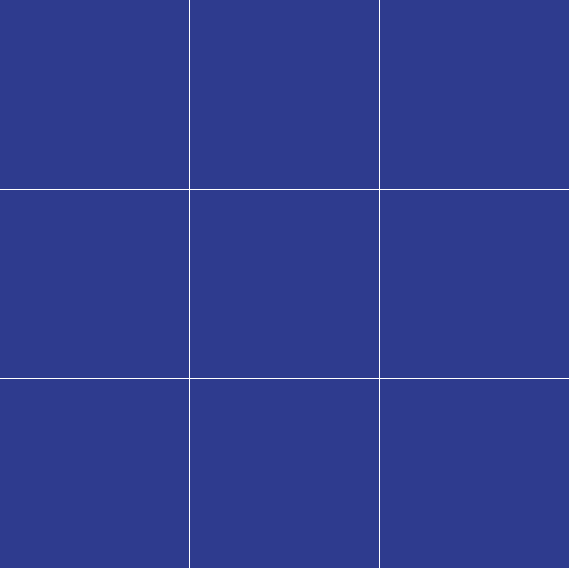
\includegraphics[width=0.3\textwidth]{3_basics/grid00.png}
  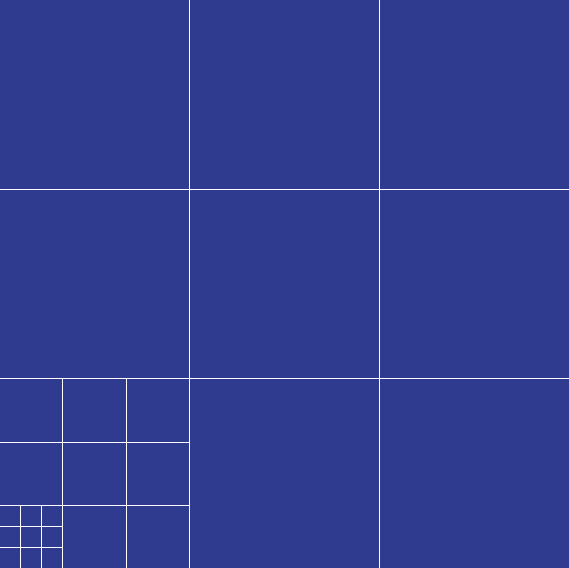
\includegraphics[width=0.3\textwidth]{3_basics/grid01.png}
  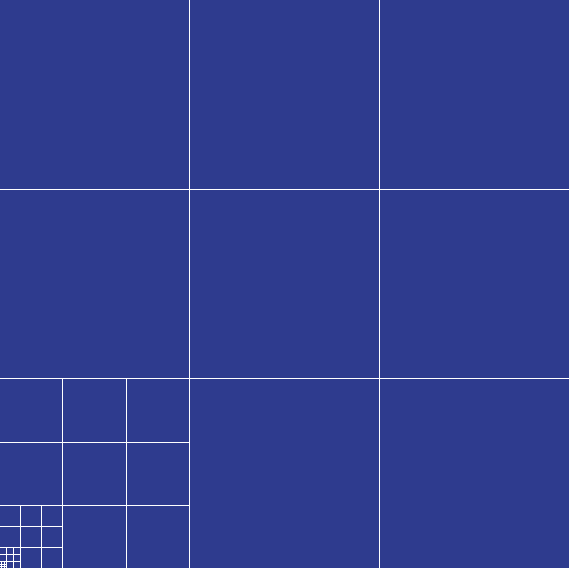
\includegraphics[width=0.3\textwidth]{3_basics/grid02.png}
\end{center}


\subsection{What happens}


\begin{center}
  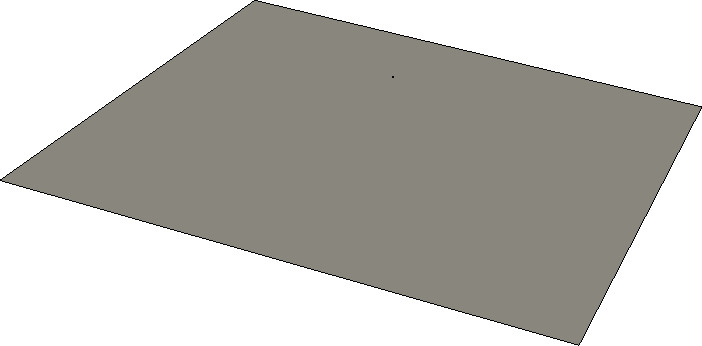
\includegraphics[width=0.45\textwidth]{3_basics/construction00.png}
  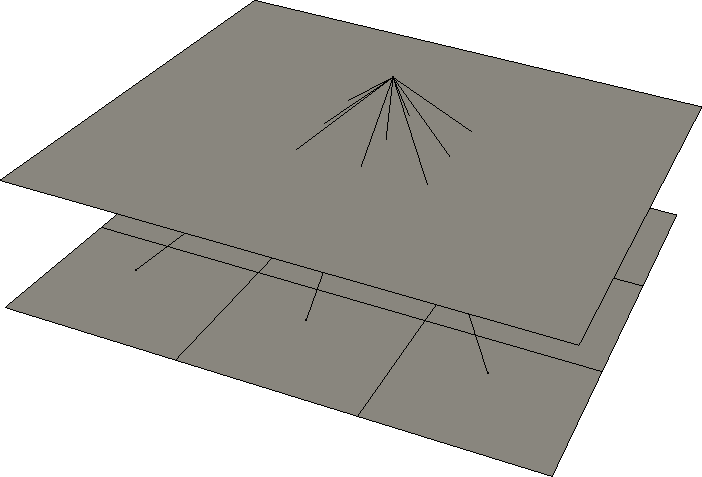
\includegraphics[width=0.45\textwidth]{3_basics/construction01.png}
  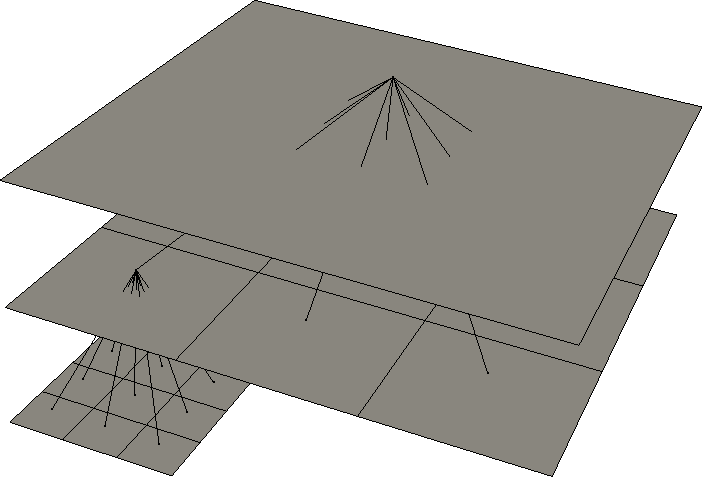
\includegraphics[width=0.45\textwidth]{3_basics/construction02.png}
  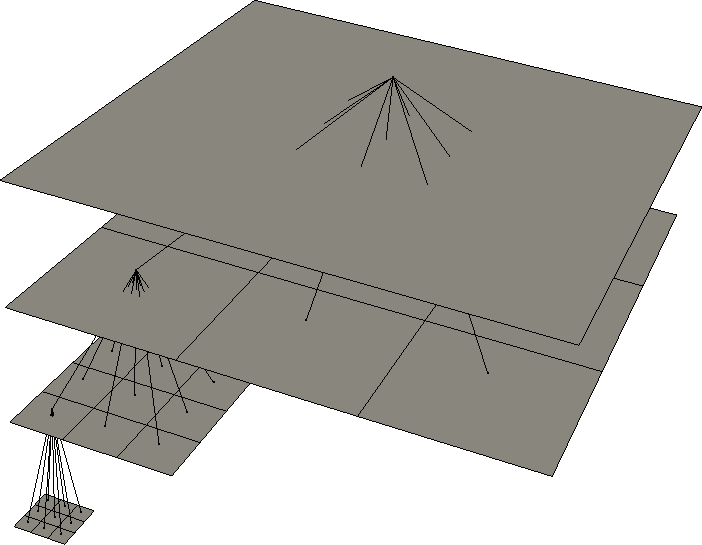
\includegraphics[width=0.45\textwidth]{3_basics/construction03.png}
\end{center}


To understand what is happening, we can read all the outputs written to the
terminal by Peano (see the next chapter how to remove them/filter them).
Or we can just give a quick sketch:

\begin{enumerate}
  \item We first create a repository. A repository is basically the spacetree,
  i.e.~the grid, plus all the adapters we've defined. It also provides some
  statistics the can read out.
  \item The code runs into the Runner's \texttt{runAsMaster()} routine and
  selects which adapter to use. This is the switch statement. In a parallel
  code, all involved ranks would now immediately active this adapter.
  \item In the runner, we then call the \texttt{iterate} operation on the
  repository. The repository now starts to run through the whole grid. Actually,
  it runs through the spacetree in a kind of top-down way.
  \item Whenever it encounters an interesting situation (it loads a vertex for
  the very first time, e.g.), it triggers an event. Event means that it calls an
  operation on the adapter.
  \item An adapter may fuse multiple events; both predefined and user-defined.
  Per event, it calls all these mappings' implementations one after another. The
  order is the same you have used in your specification file.
\end{enumerate}

\begin{remark}
  This document does not run through the list of available events, in which
  order they are called and so forth. You may want to have a look into any
  event's header. The PDT augments the header with a quite verbose explanation
  what event is called when.
\end{remark}

It might now be the right time to look into one of these mapping headers to get
a first impression what is available.
Basically, they describe all important plug-in points that you might want to use
in any element-wise multiscale grid traversal.

% 



\subsection{Multiscale data}
Prior to a discussion of Peano's data model, it might make sense to load all the
files \texttt{grid-level-?-0.vtk} into your favourite visualisation software.
Dilate them according to their level encoded in the name.
In Paraview, you have to select each file, apply
Filters/Alphabetical/Transform, and dilate each file by -0.2 along the z-axis
per level.
You might end up with something alike:



\begin{center}
  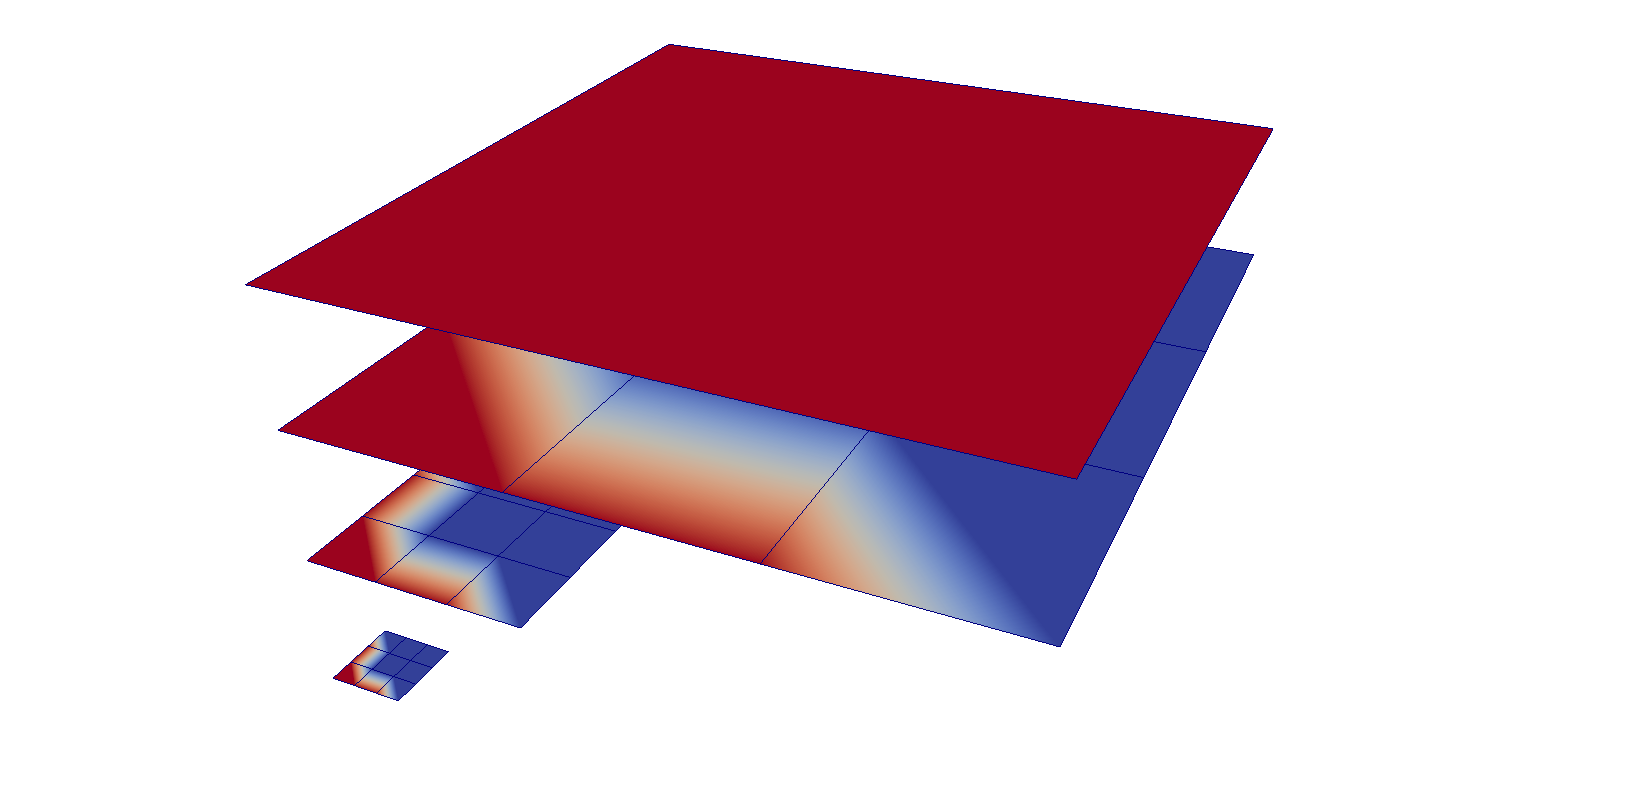
\includegraphics[width=0.8\textwidth]{3_basics/tree00.png}
\end{center}

\noindent
Again, feel free to create a video that shows how additional levels are added in
each step.
There's a more elegant way to end up with a similar picture. 
I once created a graph visualiser that is today also available as predefined
mapping. Just modify your adapters as follows:

\begin{code}
adapter:
  name: CreateGridAndPlot
  merge-with-user-defined-mapping: CreateGrid
  merge-with-predefined-mapping: VTK2dTreeVisualiser(tree,getLevel)
\end{code}

\noindent
This time, creating a video should be straightforward.
\begin{center}
  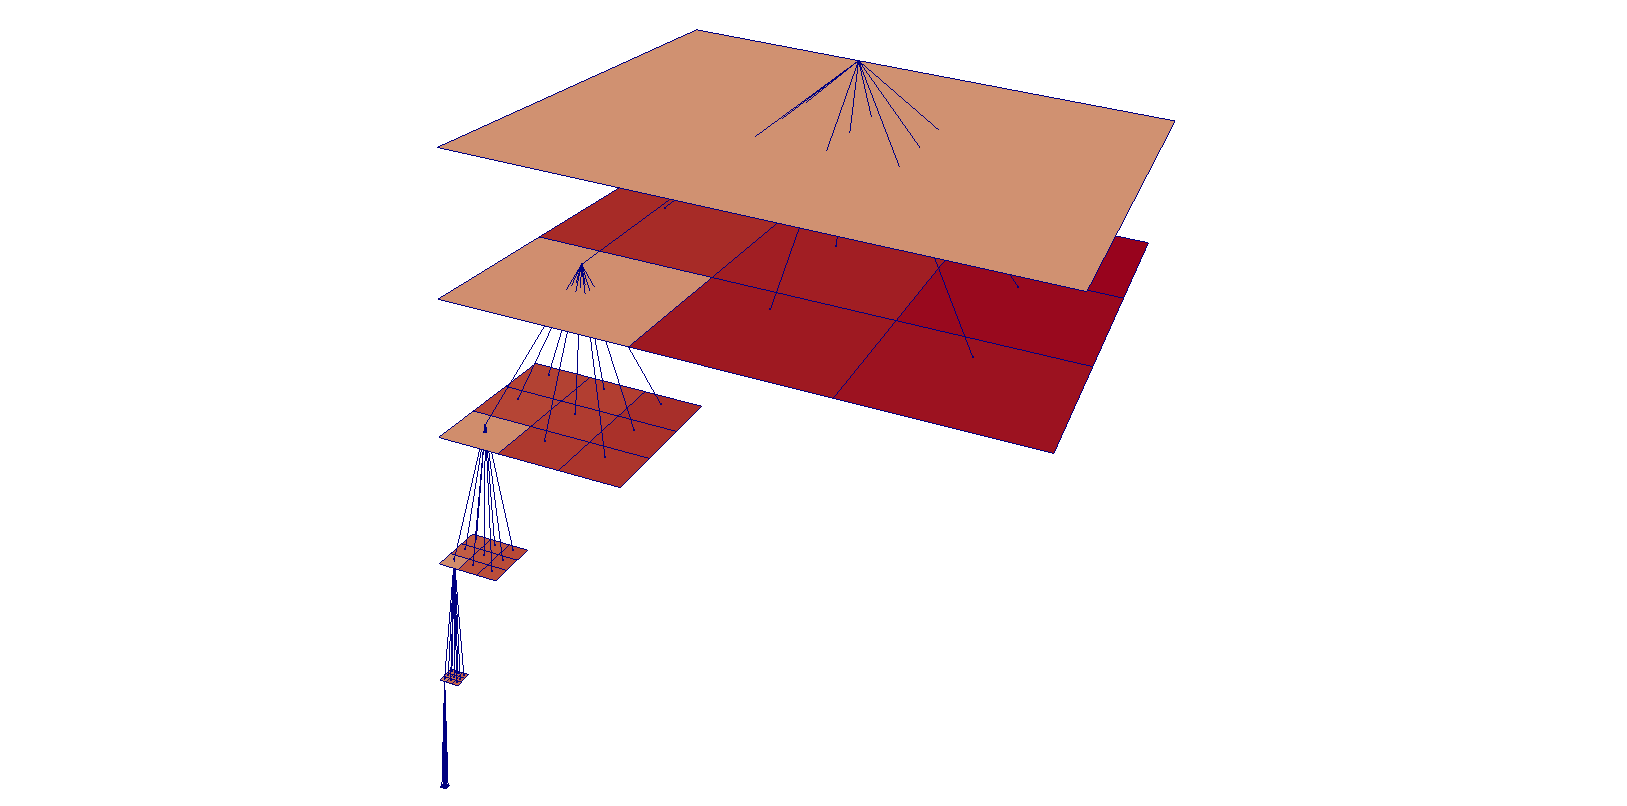
\includegraphics[width=0.8\textwidth]{3_basics/tree01.png}
\end{center}

We see that speaking of Peano in terms of a spacetree software is only one way
to go.
We also could speak of it of a software managing Cartesian grids embedded into
each other.
The latter point of view reveals an important fact:
Peano handles vertices and cells.
Cells are embedded into each other as they form the tree and there is a clear
parent-child relation.
Vertices connect cells.
A vertex is unique due to its position in space plus its level, i.e.~there might
be some coordinates that host multiple vertices.
In math, we would call this generating system.
There are two types of vertices:
the standard ones are adjacent to $2^d$ cells on the same level with $d$ being
the dimension of the problem.
All other vertices are hanging nodes.

\begin{remark}
  Hanging nodes are not stored persistently. They are created and destroyed in
  each traversal upon request and never stored in-between two iterations. You
  can never be sure how often a hanging nodes is constructed per traversal. It
  could be up to $2^d-1$ times. You only know it is created once at least.
\end{remark}

Cells and vertices hold data. This data is described in the files
\texttt{Vertex.def} and \texttt{Cell.def}.
The .def files feed into our tool DaStGen that translated them internally into a
standard C++ class (though it does some more stuff: it autogenerates all MPI
data types that we need later on for parallel codes, and it in particular
compresses the data such that a bool field is really mapped onto a single bit,
e.g.).
There's an alternative way to hold data on the grid that is called heap: in this
case, we do not assign a fixed number of properties to vertices or cells.
Both storage variants are discussed in my tech report {\em The Peano software -
parallel, automaton-based, dynamically adaptive grid traversals} which can be
obtained from arXiv, e.g.
